%
% Mars.tex
%
% History of LulzBot Printers
%
% Copyright (C) 2014, 2015 Aleph Objects, Inc.
%
% This document is licensed under the Creative Commons Attribution 4.0
% International Public License (CC BY-SA 4.0) by Aleph Objects, Inc.
%

%\begin{figure}[h!]
%\includegraphics[keepaspectratio=true,height=0.40\textheight,width=1.00\textwidth,angle=0]{mars/mars-display.jpg}
% \caption{LulzBot Mars.}
% \label{fig:taz-display}
%\end{figure}

The first two printers in the LulzBot 3D Printer cluster were Prusa
RepRaps put together with printed parts purchased off the Internet.
They were built in the first quarter of 2011.
These two printers printed the next set of parts needed by the
subsequent LulzBot Prusa Clonedels.

%
% Mars.tex
%
% History of LulzBot Printers
%
% Copyright (C) 2014, 2015 Aleph Objects, Inc.
%
% This document is licensed under the Creative Commons Attribution 4.0
% International Public License (CC BY-SA 4.0) by Aleph Objects, Inc.
%

\section{Prusa Mars P1}
Prusa Mars P1.

\begin{figure}[h!]
\thisfloatpagestyle{empty}
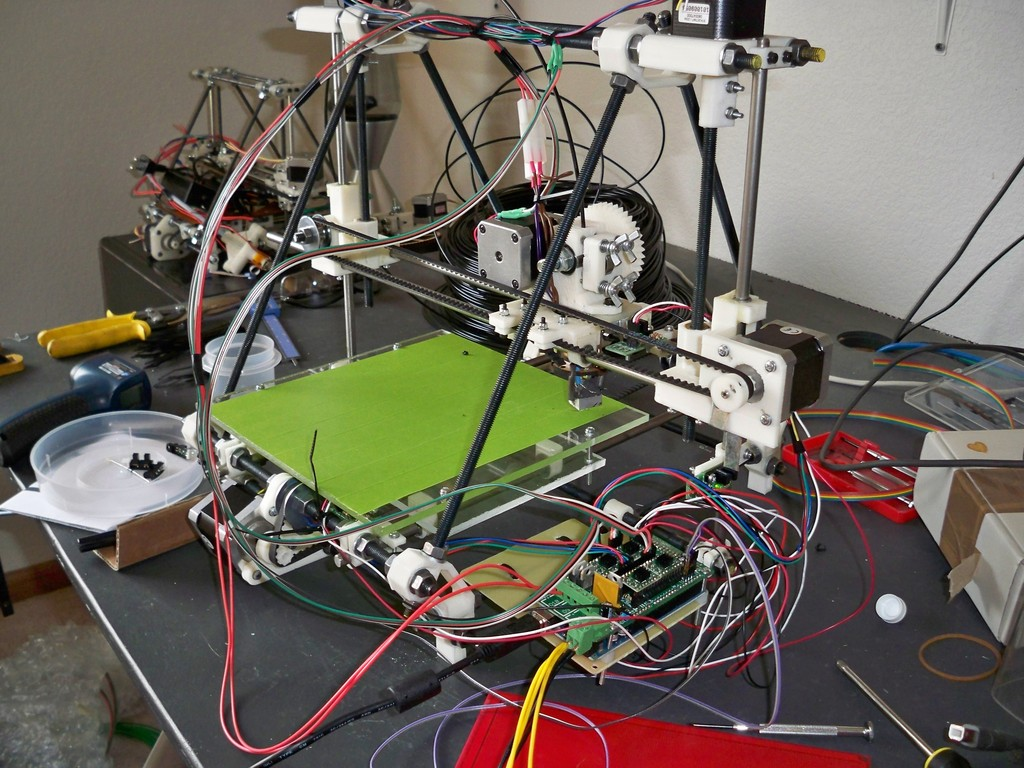
\includegraphics[keepaspectratio=true,height=0.40\textheight,width=1.00\textwidth,angle=0]{mars/mars-p1.jpg}
 \caption{LulzBot Mars P1.}
 \label{fig:mars-p1}
\end{figure}


%
% Mars.tex
%
% History of LulzBot Printers
%
% Copyright (C) 2014, 2015 Aleph Objects, Inc.
%
% This document is licensed under the Creative Commons Attribution 4.0
% International Public License (CC BY-SA 4.0) by Aleph Objects, Inc.
%

\section{Prusa Mars P2}
Prusa Mars P2.

\begin{figure}[h!]
\thisfloatpagestyle{empty}
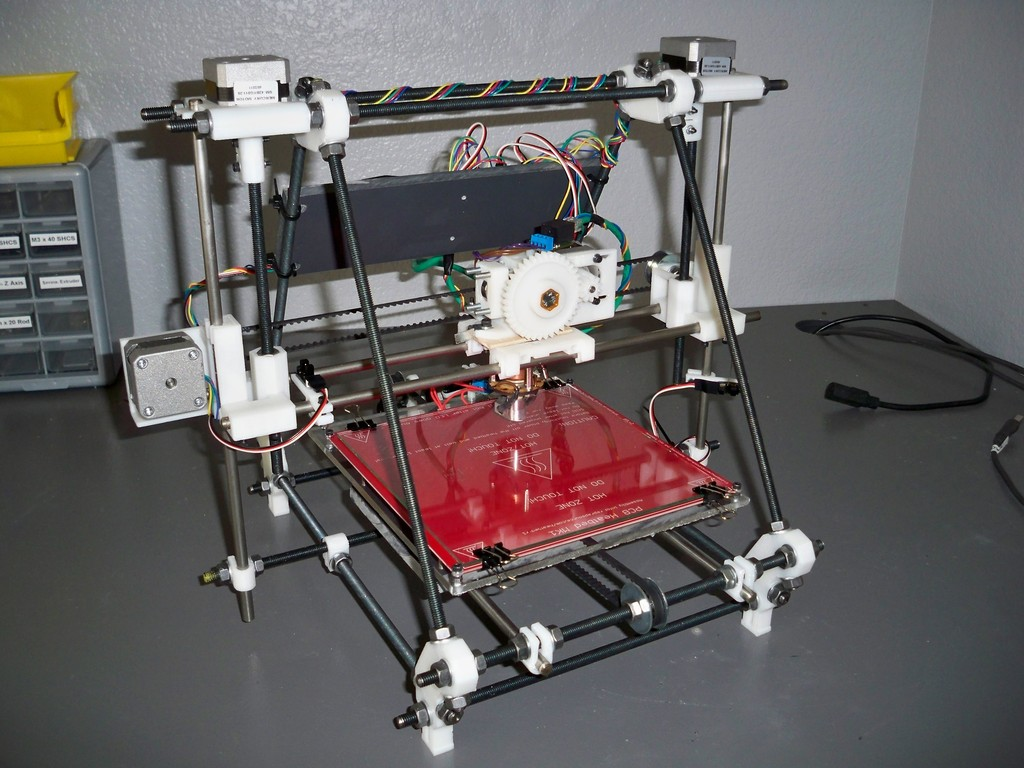
\includegraphics[keepaspectratio=true,height=0.40\textheight,width=1.00\textwidth,angle=0]{mars/mars-p2.jpg}
 \caption{LulzBot Mars P2.}
 \label{fig:mars-p2}
\end{figure}



% It is unknown who printed the parts for Mars P1 & P2. The parts were white.
% These are the most likely:
% PO00057 - 2011-01-25 - Anthony Quan - ebay 190494251338 - 
% PO00053 - 2011-01-26 - Jonathan Botelho - eBay 220729673538 - 
% PO00055 - 2011-01-26 - eMakershop - 
% PO00056 - 2011-01-26 - eMakershop - 
%
% The sets below are known to *NOT* to have been used,
% because of color (Mars P1 & P2 were both white):
% aachen_2011 (is this an ebay alias?) - Not white.
% Nicholas RepRap Breeding project - Light blue PLA parts.
% PO00058 - 2011-01-27 - MAKER FARM INC., Colin Farrer - eBay 230574968489 - elderfarrer2hy7 - Black parts.

